\section{Execution}
\label{sec:Durchführung}
The experiment is carried out with the D8 laboratory diffractometer from Brunker-AXS \cite{V44} (shown in \autoref{fig:experiment}). 
\begin{figure}
  \centering
  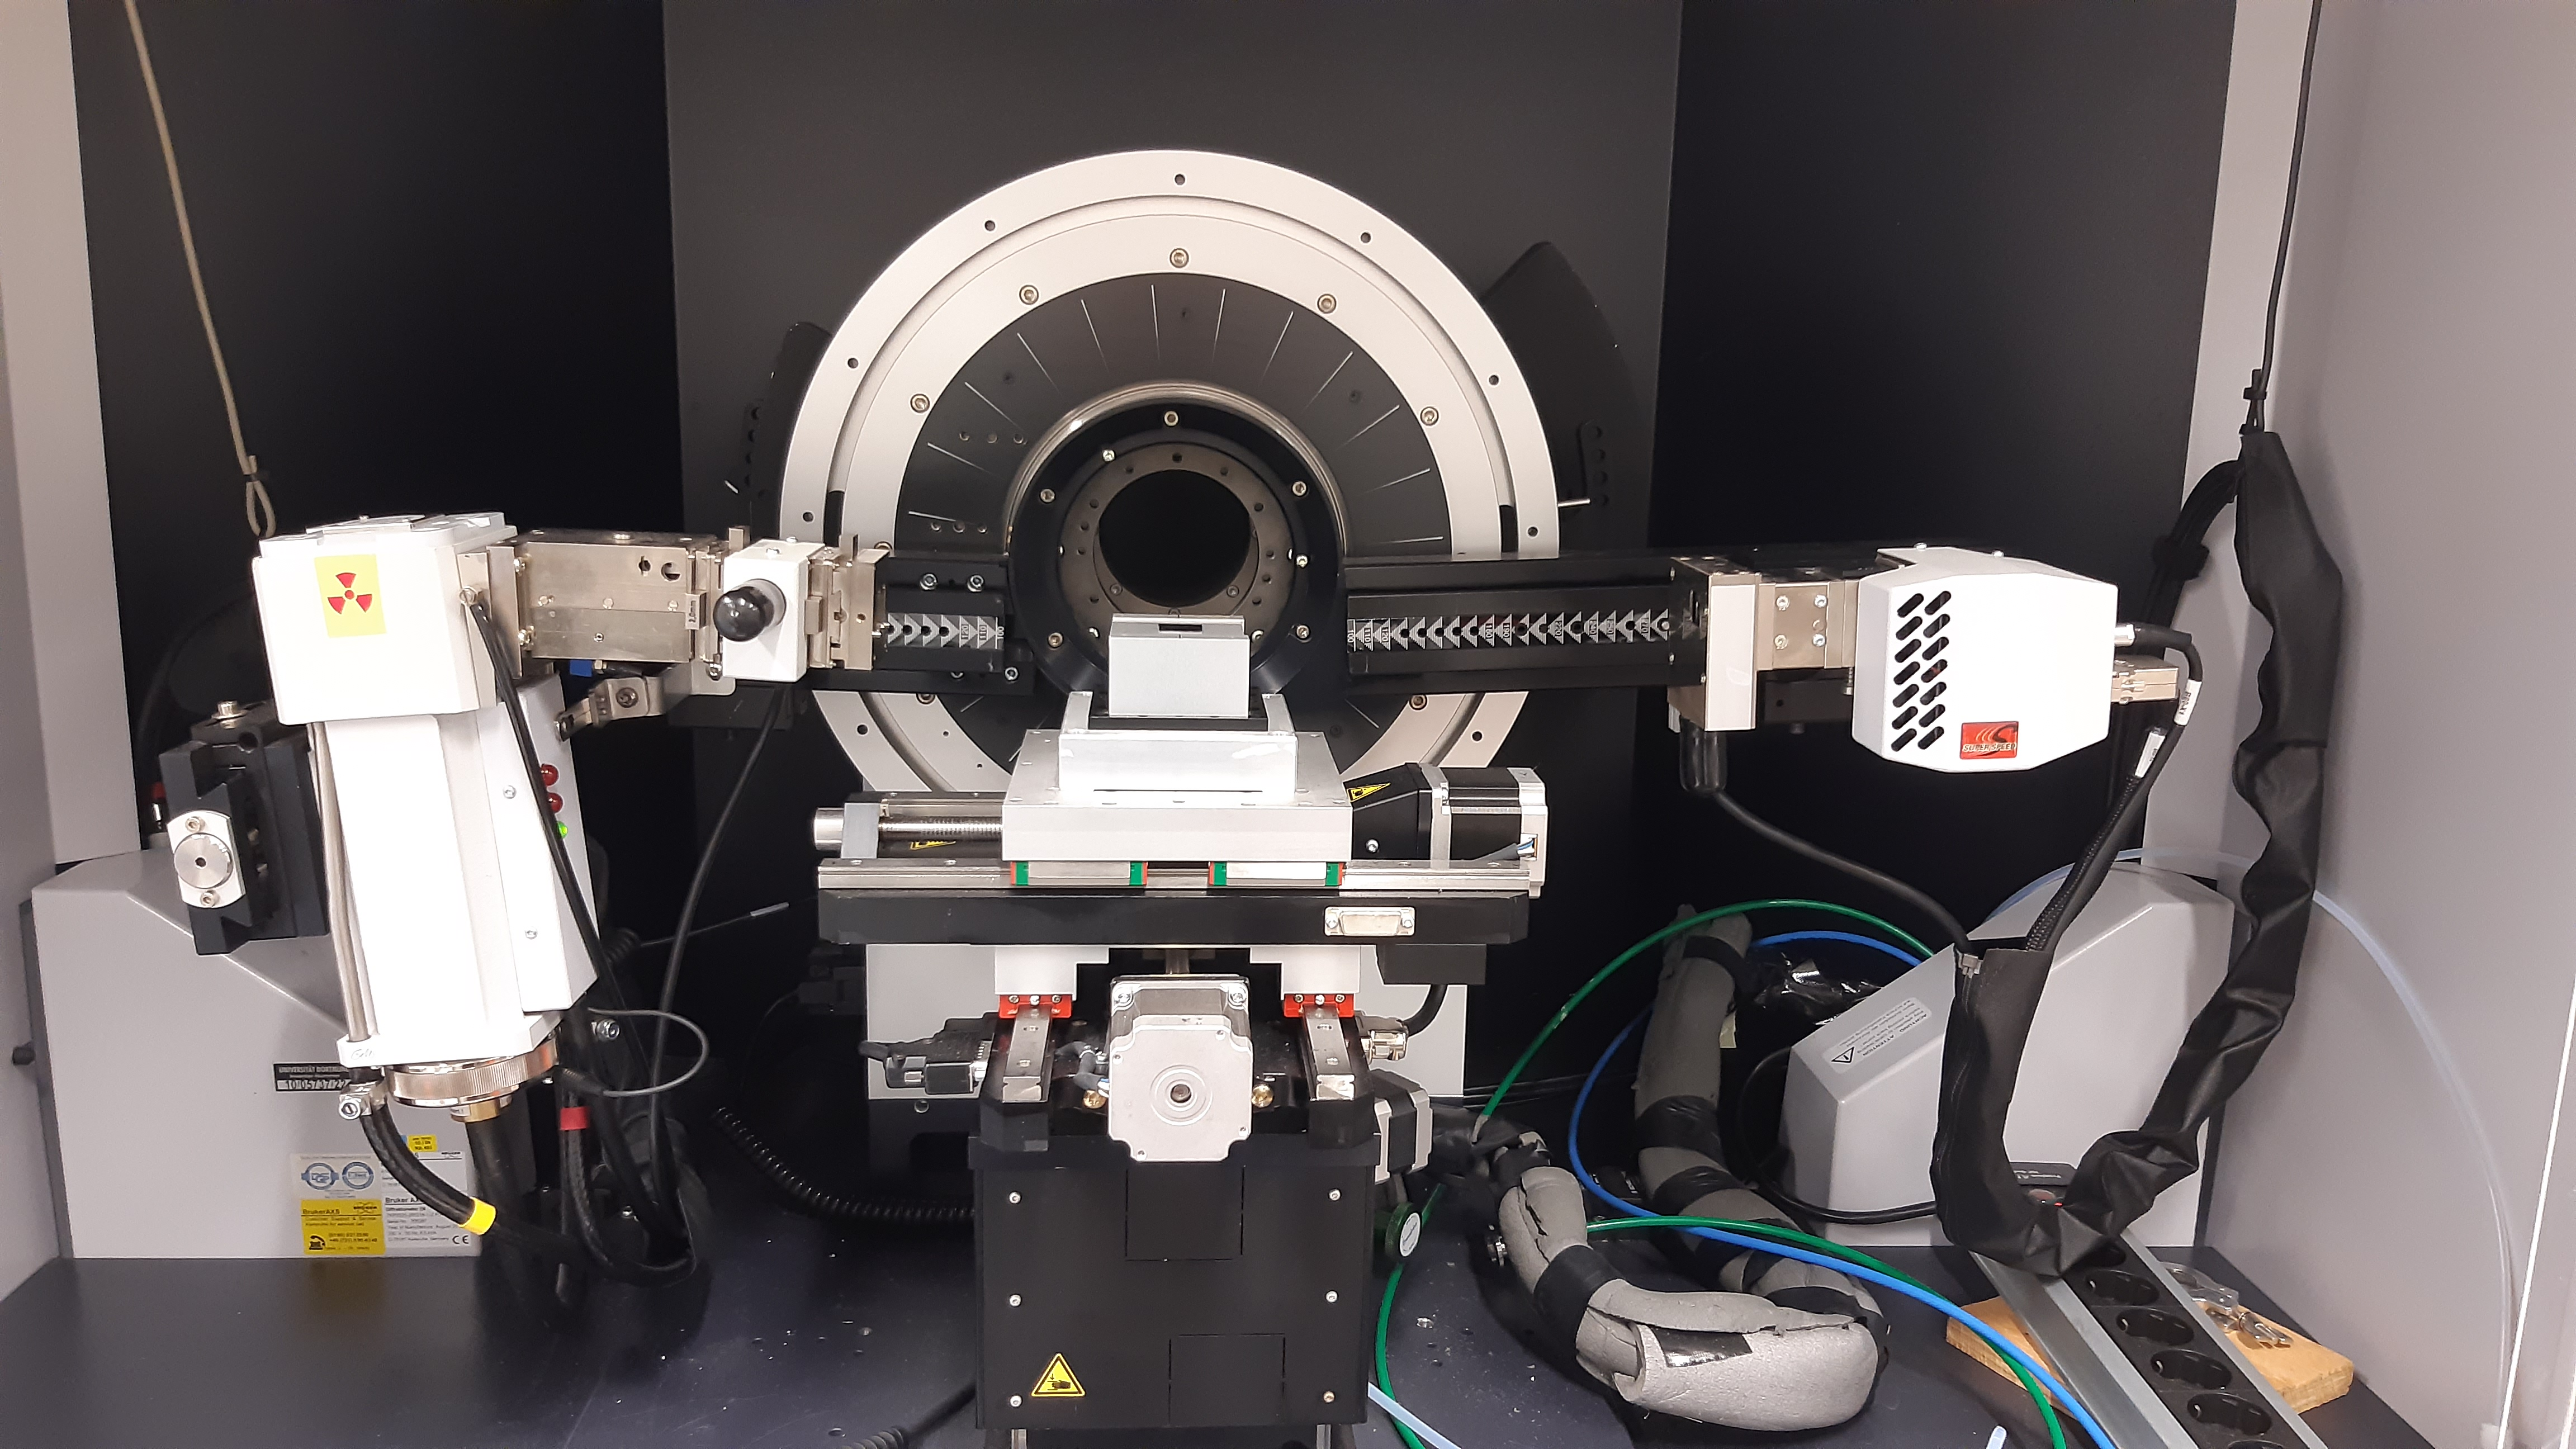
\includegraphics[width=0.8\textwidth]{images/aufbau.jpg}
  \caption{Setup of the experiment.}
  \label{fig:experiment}
\end{figure}
The x-ray radiation is emitted by the copper tube, shown in \autoref{fig:source}.
\begin{figure}
  \centering
  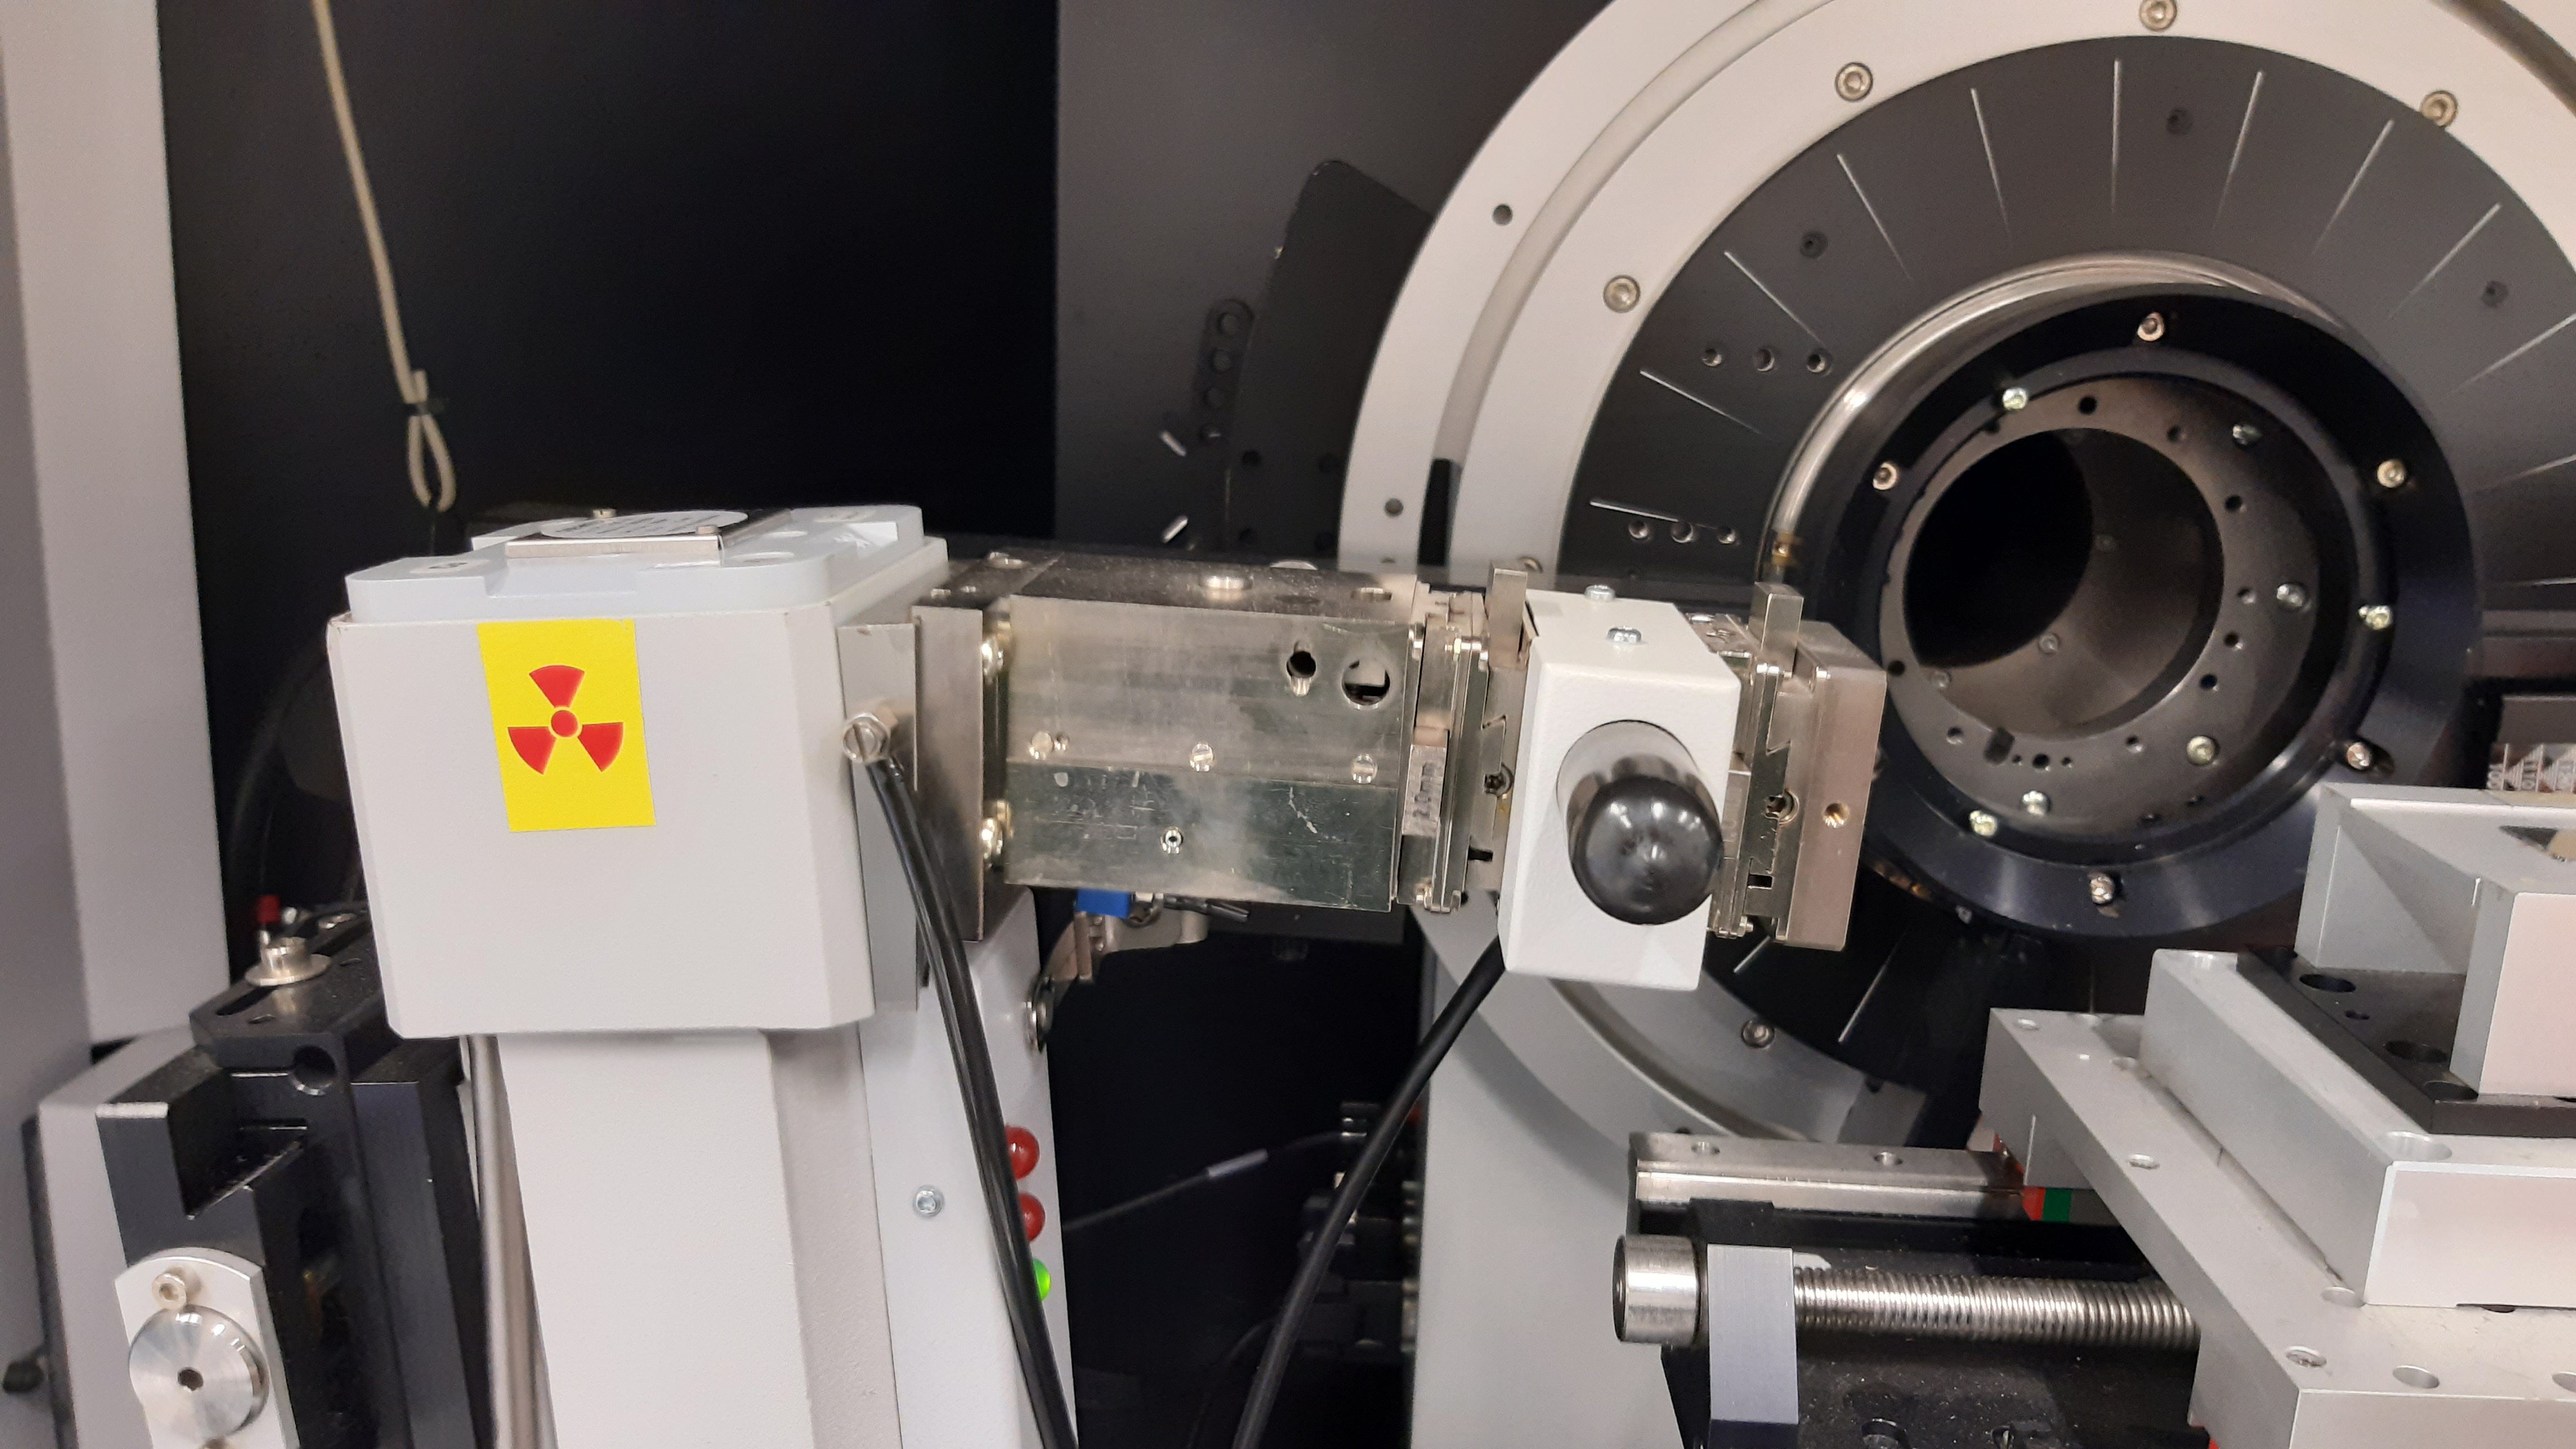
\includegraphics[width=0.8\textwidth]{images/quelle.jpg}
  \caption{X-ray source on the left.
  In the middle is the Göbel mirror.}
  \label{fig:source}
\end{figure}
The radiation falls on the Göbel mirror and gets reflected onto the probe.
The Probe is fixated on a movable table, shown in \autoref{fig:probe}.
The intensity of the reflected radiation is measured with a detector, shown in \autoref{fig:detector}. 
\begin{figure}
  \hfill
  \begin{subfigure}{0.46\textwidth}
    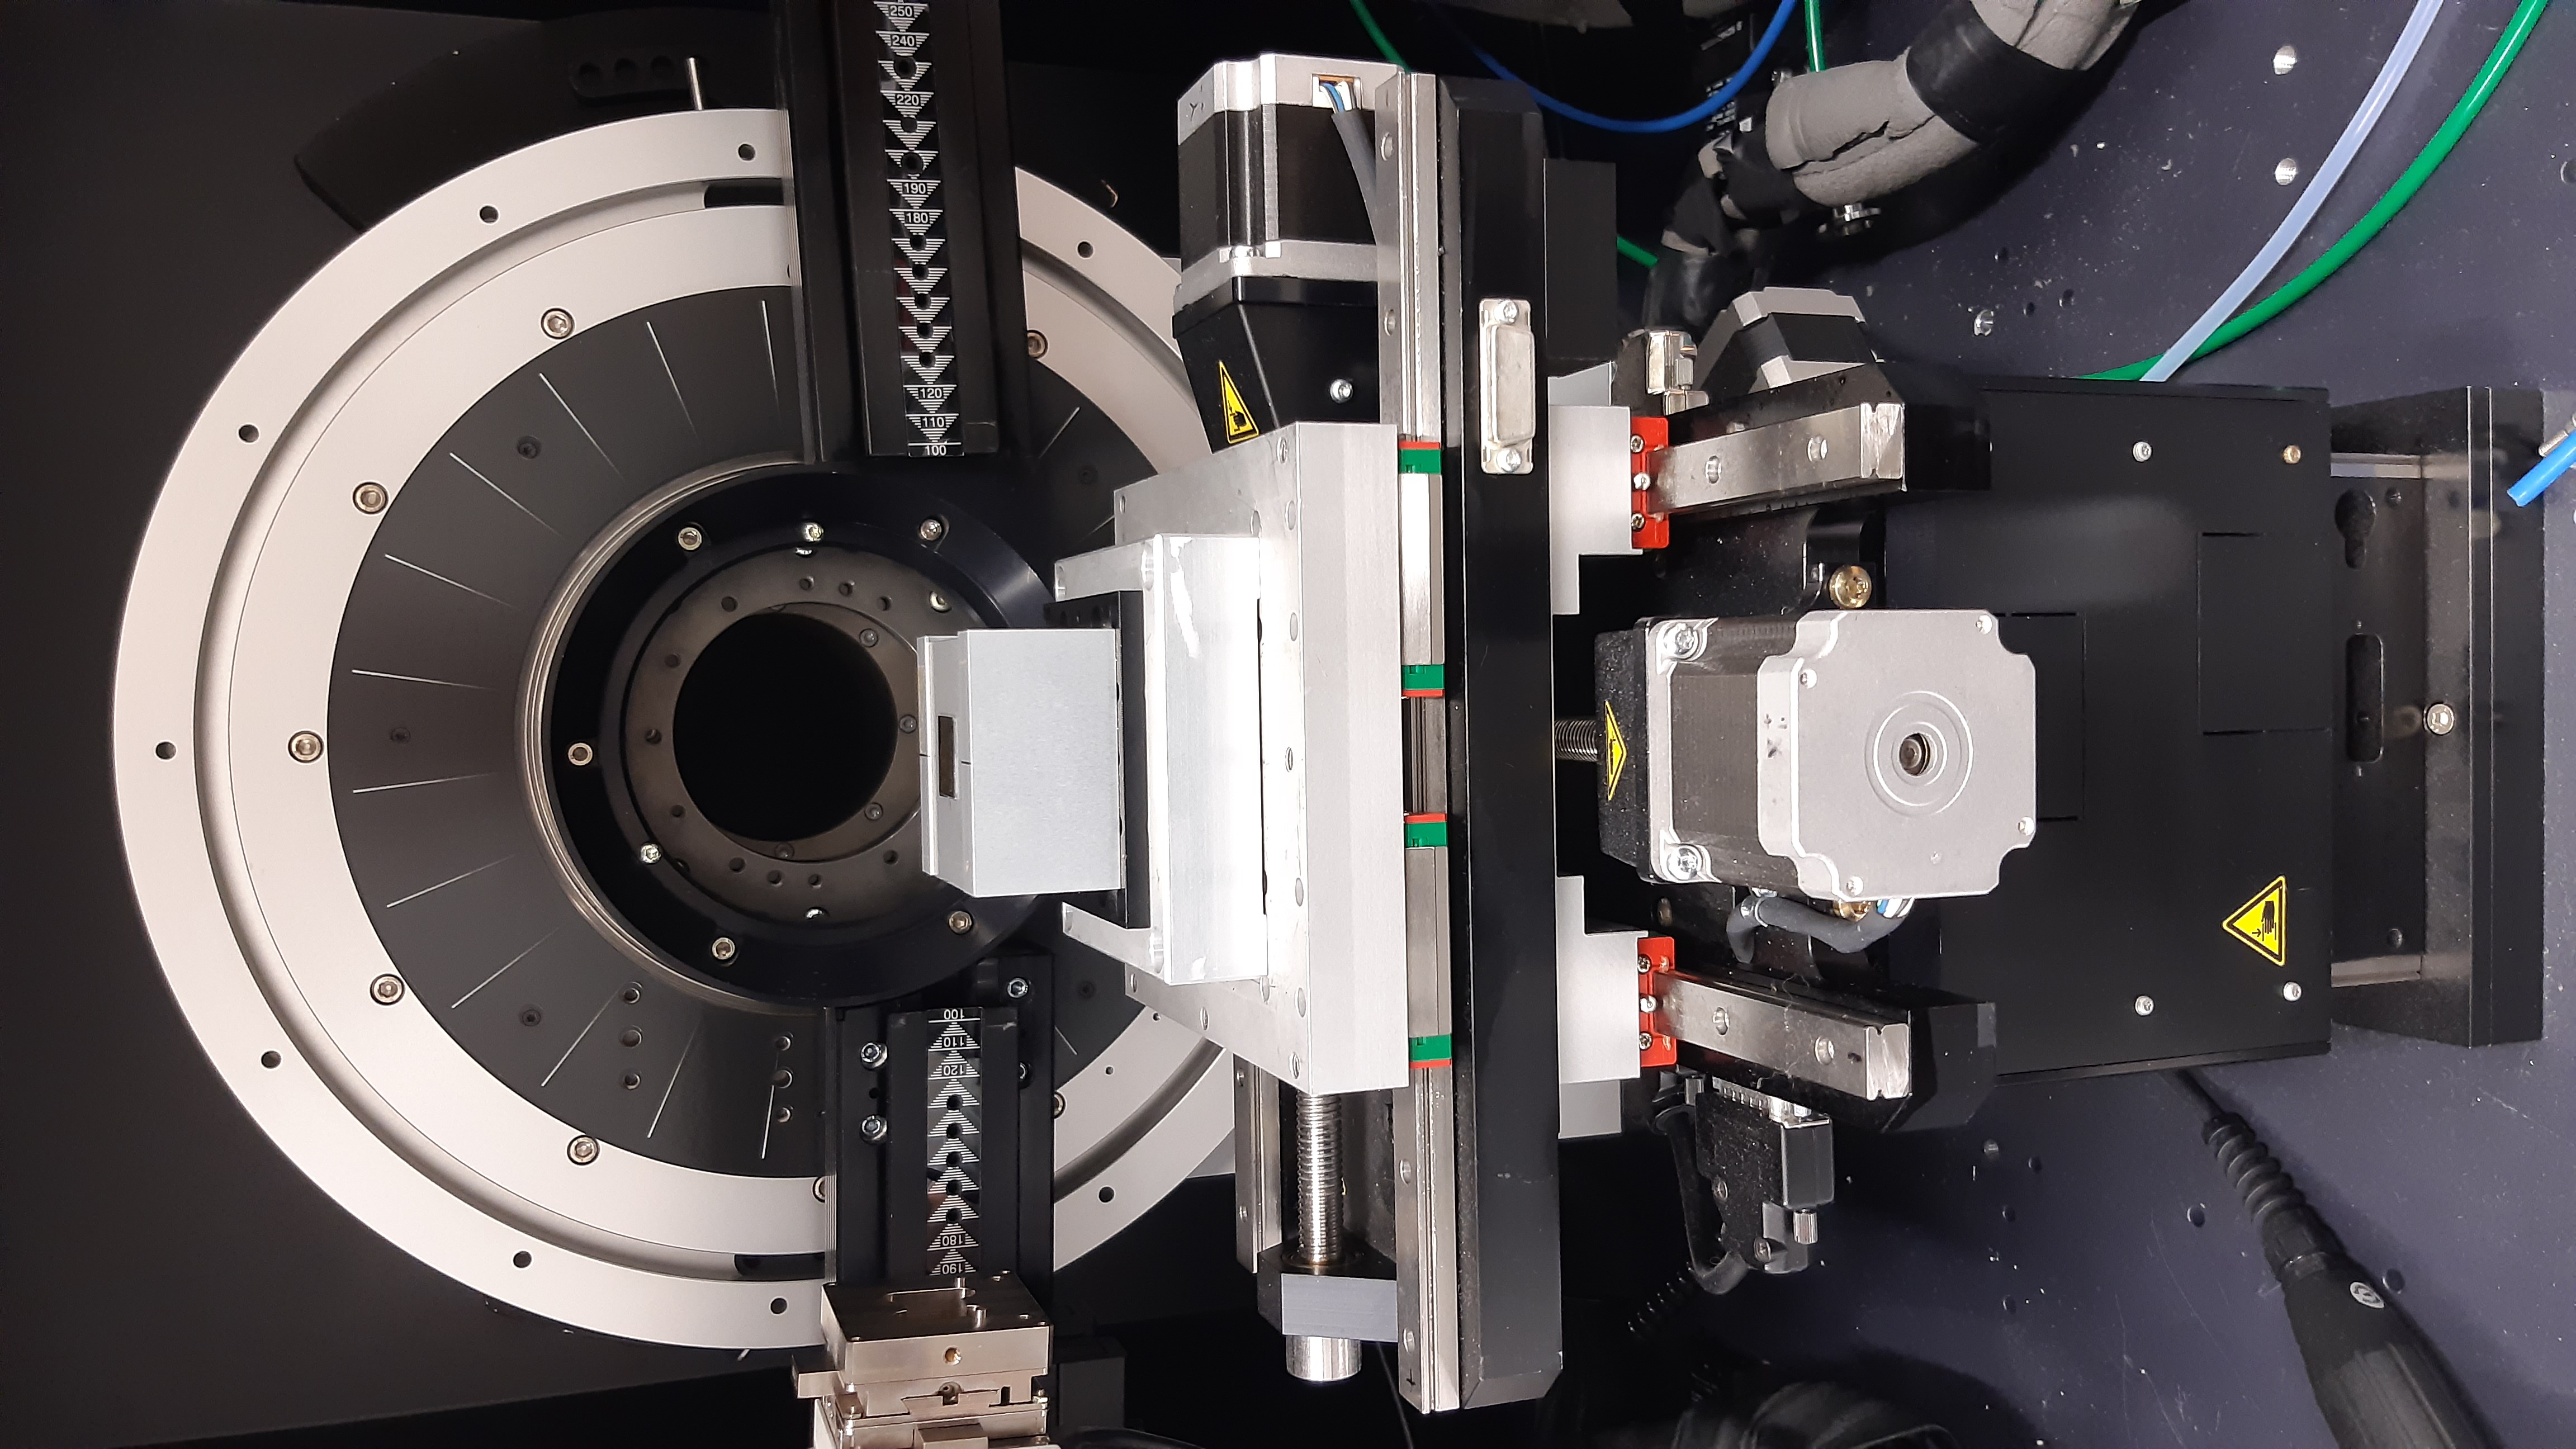
\includegraphics[width=\textwidth, angle=270]{images/probe.jpg}
    \caption{Probe on movable table.}
    \label{fig:probe}
  \end{subfigure}
  \hfill
  \begin{subfigure}{0.46\textwidth}
    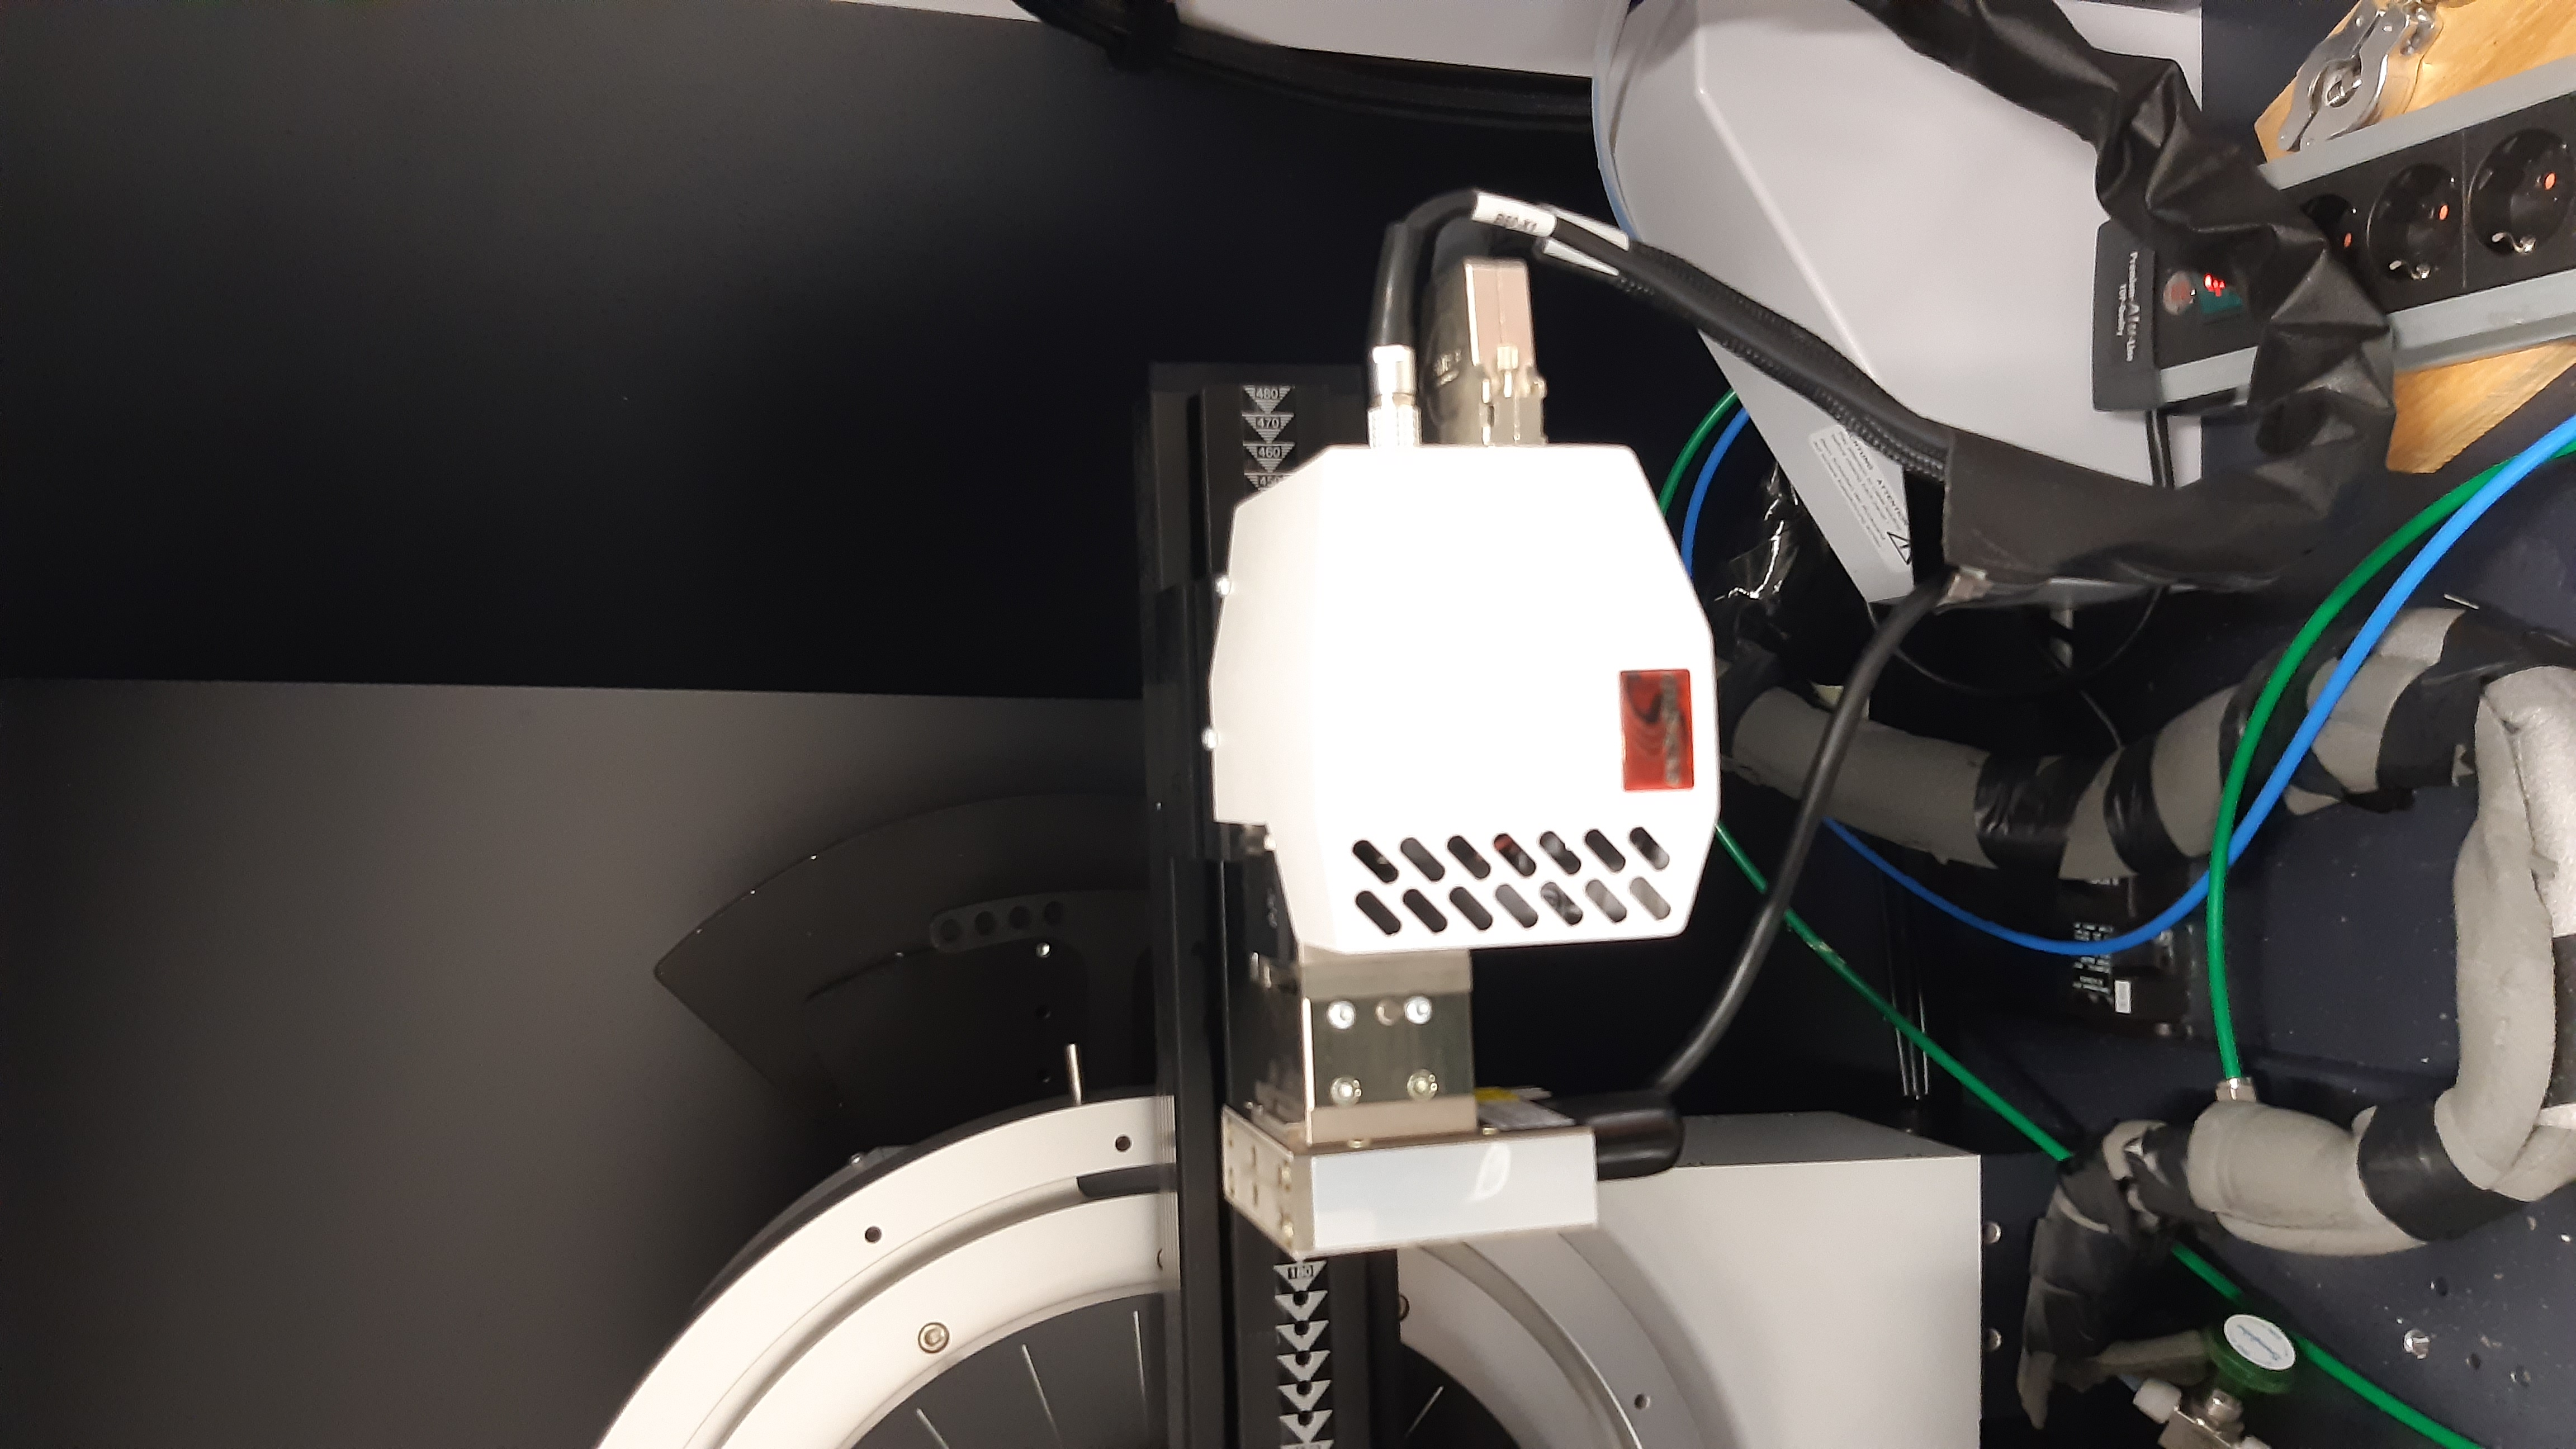
\includegraphics[width=\textwidth, angle=270]{images/detektor.jpg}
    \caption{Detector for x-ray radiation.}
    \label{fig:detector}
  \end{subfigure}
  \caption{Probe and detector.}
  \hfill
\end{figure}

Before the measurement can start the experiment has to be adjusted.
At the beginning, the detector must be adjusted. To do this, the stage with the sample is lowered and the radiation source is directed directly at the detector. this is to ensure that the detector and the source are aligned in the same way.
Then the $z$-coordinate (height coordinate) is adjusted. For this purpose, the stage is moved up so that half of the intensity of the beam is covered by the stage and the sample.
The $x$-axis is then adjusted. Here, it is basically unimportant on which area of the specimen the beam falls, as long as the entire beam is reflected by the sample.
Now the $y$-axis is adjusted. This adjustment compensates for small misalignments, such as tilting, of the sample.

Now the $z$-axis is readjusted again, since the optimum position may have changed as a result of the previous adjustment steps. In addition, another rockingscan is performed.
To further improve the precision of the measurement, another scan of the $z$-axis and a rockingscan are performed at an inclination of the source and the detector of $2\theta=0.3$ and $2\theta=0.5$ respectively.

\begin{table}
  \centering
  \caption{Adjustment steps with their respective values \cite{V44}.}
  \label{tab:adjustment}
  \begin{tblr}{
    colspec={l S[table-format=-2.1] S[table-format=2.1] S[table-format=1.3] S[table-format=1.2]},
    row{1}={guard},
    vline{3}={2}{-}{text=to},
    }
    \toprule
    \SetCell{c} Scan type & \SetCell[c=2]{c} Range & & Step size & $2\theta\mathbin{/}\unit{\degree}$ \\
    \midrule
    Detector scan &  -0.5 &  0.5 & 0.02  & 0.0 \\
    $z$ scan      &  -1.0 &  1.0 & 0.04  & 0.0 \\
    $x$ scan      & -20.0 & 20.0 & 1.00  & 0.0 \\
    Rockingscan   &  -1.0 &  1.0 & 0.04  & 0.0 \\
    $z$ scan      &  -0.5 &  0.5 & 0.02  & 0.0 \\
    Rockingscan   &   0.0 &  0.3 & 0.005 & 0.3 \\
    $z$ scan      &  -0.5 &  0.5 & 0.02  & 0.3 \\
    Rockingscan   &   0.2 &  0.5 & 0.005 & 0.5 \\
    \bottomrule
  \end{tblr}
\end{table}

After the adjustment, the measurement can begin. The measurement type is the \textbf{Omega/2Theta} scan.
It is measured from $\qty{0}{\degree}$ to $\qty{2.5}{\degree}$, with a step size of $\qty{0.005}{\degree}$.
For each step, the measurement is taken for $\qty{5}{\second}$.
Afterwards the same measurement is performed again, but with the difference that the angle of the detector is shifted by $\qty{0.2}{\degree}$.
Thus the diffuse background radiation is measured, with which the real measurement can be corrected afterwards.